\documentclass{article}
\usepackage{listings}
\usepackage{graphicx}

\newcommand{\SolutionName}{BinarySearch}
\newcommand{\ProjectName}{BinarySearch}

\newcommand{\code}[1]{\lstinline{#1}}

\title{\ProjectName{} Static Checking Example}
\date{}


\begin{document}
\maketitle
\begin{abstract}
This example shows checking of implicit non-null requirements as well
as array indexing requirements. The example consists of a binary
search routine and a small client of the search that increments a
value inside an array. To find the proper place to increment, it
searches for the value first.
\end{abstract}

\newcommand\codefamily\sffamily
\lstset{language={[Sharp]C},mathescape=true,flexiblecolumns=true,morekeywords={Requires,Ensures,Invariant},basicstyle=\codefamily\small,literate={->}{{$\rightarrow$}}{2}{<<}{{$\langle$}}{2}{>>}{{$\rangle$}}{2}{!}{{\textbf{!}}}{2},frame=lines,moredelim=[is][\itshape]{@}{@},captionpos=b,numberstyle=\tiny,stepnumber=1,numbersep=2pt}

\section{Adding the Contract Library Reference}
If you are using Visual Studio 2008, or if you for 
some reason want to target a pre-v4 .NET runtime, then you need to:
\begin{itemize}
\item Change the target framework of the project.
\item Manually add a reference to Microsoft.Contracts.dll
\end{itemize}
Otherwise, you may skip this section and go directly the next section!

To add the reference, open the
\textsf{\SolutionName{}} solution and right-click on
\textsf{References} in the \textsf{\ProjectName{}} project and
select \textsf{Add Reference}. Find the \textsf{Microsoft.Contracts}
library in the \textsf{.NET} tab as shown below and click OK.
\begin{center}
  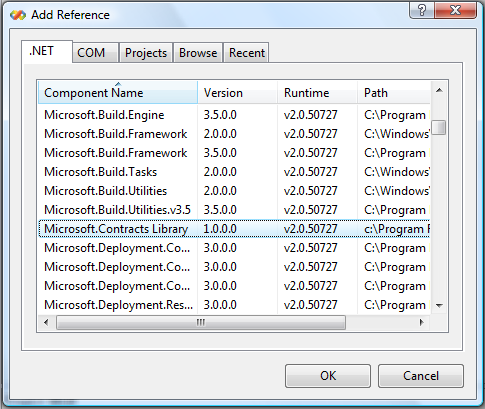
\includegraphics[width=.7\columnwidth]{../Common/addRef.png}
\end{center}



\section{Sample Walkthrough}
\label{sec:start}

After adding the proper reference, go to the Properties of project
\textsf{\ProjectName}, select the Code Contracts pane (at the bottom), and enable static
checking by clicking on the static checking box. Also enable implicit
non-null and array checks, as shown in this screenshot:
\begin{center}
  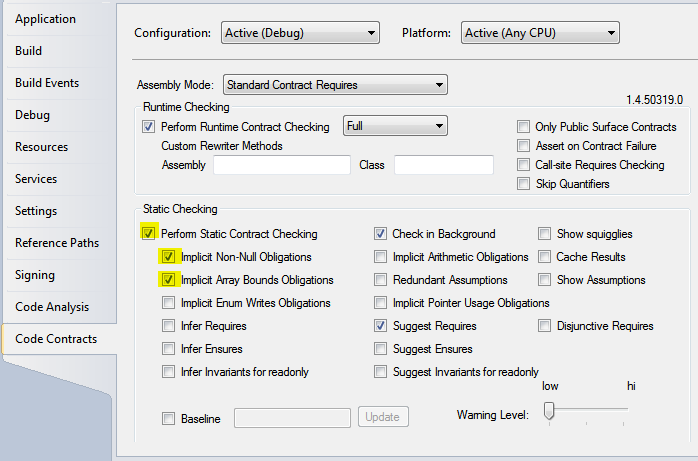
\includegraphics[width=.8\columnwidth]{ex1.png}
\end{center}

Then build the example. The build should succeed. After a
moment\footnote{The static checker runs in the background after the regular build.}, 
the static checker should warn about the
following problems:
\begin{center}
  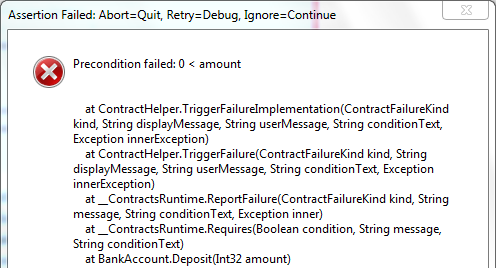
\includegraphics[width=1\columnwidth]{ex2.png}
\end{center}
The first, second, and fourth errors are all reported in the \code{IncrementIndex} method
and have to do with the fact that the method assumes that the \code{array}
passed as a parameter is non-null. Similarly, it assumes that the index
is within the array. The static checker tells us that we should make
these assumptions explicit as contracts. If you switch to the Messages
tab in Visual Studio, you see that the checker actually
suggests the proper preconditions:
\begin{center}
  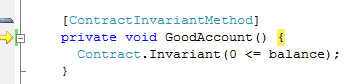
\includegraphics[width=1\columnwidth]{ex3.png}
\end{center}
Add those preconditions to the \code{IncrementIndex} method (remember
to use the \textsf{cr TAB TAB} abbreviation in C\# to insert Requires):
\begin{lstlisting}
  Contract.Requires(array != null);
  Contract.Requires(0 <= index);
  Contract.Requires(index < array.Length);
\end{lstlisting}
If we build again, we get a number of new warnings. Let's fix the one
in \code{BinarySearch} on line 14 first, as it is similar to the ones
we just did. The \code{BinarySearch} method assumes that the passed
\code{array} is non-null and we make that explicit using a
precondition:
\begin{lstlisting}
  public static int BinarySearch(int[] array, int value)
  {
    Contract.Requires(array != null);
\end{lstlisting}
After rebuilding again, the remaining warnings are all in method
\code{IncrementValue}. Here, the checker cannot ascertain the
preconditions of our calls to \code{BinarySearch} and
\code{IncrementIndex}. Note that it does not warn about the first
precondition \code{array != null} in \code{IncrementIndex} again, as
the checker determines that given the fact that it should be non-null
in the call to \code{BinarySearch}, it would still be non-null in the
call to \code{IncrementIndex}.

The nullness error is again easy to fix by simply adding
\begin{lstlisting}
  Contract.Requires(array != null);
\end{lstlisting}
Because this is such a common precondition, there is a special C\#
abbreviation for it: \textsf{crn TAB TAB}. To get rid of the remaining
errors, we have to make it explicit that the \code{BinarySearch}
method actually returns an index into the searched array, so let's add
that as a postcondition to \code{BinarySearch}.
\begin{lstlisting}
  Contract.Ensures(Contract.Result<int>() >= 0);
  Contract.Ensures(Contract.Result<int>() < array.Length);
\end{lstlisting}
Note that you can use the C\# abbreviation \textsf{ce TAB TAB} to get
a postcondition, and within that postcondition, use \textsf{crr TAB
  TAB} to get the expression to refer to the method result.

Rebuild the project to see if we got everything right. Lo and behold,
there is still an error. The checker should point you at the
\code{return -1} in the \code{BinarySearch} body. Clearly, our
postcondition is too strong in that the method does not always return
an index into the array, namely when the value is not found. In that
case, it returns -1. So let's weaken the postcondition to the
following:
\begin{lstlisting}
public static int BinarySearch(int[] array, int value)
{
  Contract.Requires(array != null);
  Contract.Ensures(Contract.Result<int>() >= -1);
  Contract.Ensures(Contract.Result<int>() < array.Length);
\end{lstlisting}
and build again. Surely now we must be done ;-) But no, the checker
finds yet another problem. It complains that the call to
\code{IncrementIndex} in the \code{IncrementValue} method does not
satisfy the precondition \code{index >= 0}. Obviously, the
\code{IncrementValue} method is not handling the case where the
element is not present in the array. We fix the code by adding a test
after the \code{BinarySearch} call:
\begin{lstlisting}
public static void IncrementValue(int[] array, int val)
{
  Contract.Requires(array != null);
  
  int i = Search.BinarySearch(array, val);

  if (i == -1)
  {
    // not found
    return;
  }

  IncrementIndex(array, i);
}
\end{lstlisting}
Finally, a rebuild will confirm that we now handled the corner
cases. One final thing to point out is that the checker figured out
the safety of the array indexing operations within the
\code{BinarySearch} automatically, by inferring the necessary loop
invariant.

\end{document}
